\title{RADseq Works in Primates, Dammit.}
\author{
        Christina M. Bergey
			\and
			Andrew S. Burrell
			\and
			Luca S.J. Pozzi
			\and
			Todd R. Disotell
	}
\date{\today}

\documentclass[12pt]{article}

\usepackage{color}
\usepackage{graphics}

\begin{document}
\maketitle

\begin{abstract}
\ldots Blah, blah, blah, RADseq, blah, blah, Cercopithecoidea. \ldots
\end{abstract}

\section{Introduction}
\begin{itemize}
	\item Next-gen sequencing revolution promises gains in primatology
	\item Still expensive
	\item Many genomes, but still tough doing genomics on non-model organisms
	\item What is RADseq?
	\item Previous RADseq studies
	\item Why would it be good for primates
	\item PRESENT STUDY
	\begin{itemize}
		\item We did RADseq on 6 Cercopithecoids
		\item Assessed how well it worked
		\item Show it has promise for primates
	\end{itemize}
\end{itemize}

\section{Methods}

\paragraph{Library Preparation and Sequencing}

	Genomic DNA from 6 primates was digested with \emph{PspXI} (New England Biolabs) and used to create a multiplexed RAD tag library. Our library preparation method followed that of Etter et al, 2011 with the following modifications: the P1 adapter top\textcolor{red}{(?)} oligonucleotide was modified to have an overhang corresponding to the cut site of \emph{PspXI}, and a longer P2 adapter suitable for paired end sequencing was used (P2\_top: 5'-\textcolor{red}{SEQUENCEHERE}-3'; P2\_bottom: 5'-\textcolor{red}{SEQUENCEHERE}-3'). Individual-specific barcodes contained in the P1 adapter differed by at least \textcolor{red}{three} nucleotides. We chose \emph{PspXI} based on the results of \emph{in silico} digestion of the human, rhesus macaque, and baboon reference genomes using custom Perl scripts (\textcolor{red}{refs}). We sequenced the prepared library as one 150-cycle paired-end run of an Illumina MiSeq at the NYU Langone Medical Center's Genome Technology Center using a spike-in of 30\% PhiX DNA to control for low diversity in the library at the barcode and restriction sites. Other individuals were sequenced alongside those of the present study. Sequences are available to download from the NCBI Short Read Archive (accession number \textcolor{red}{SRAXXXXXX.X}).

\paragraph{Sequence Analysis}

	Sequence reads were demultiplexed, or separated by barcode, and reads without an expected barcode or an intact restriction enzyme cut site were excluded from the analysis. Reads were then aligned to the rhesus macaque reference genome (v.1.0, Mmul\_051212/rheMac2, \textcolor{red}{ref}) using BWA with default parameters. Reads that were unmapped, unpaired, duplicates, or that had low mapping quality were removed after alignment using Picard (\textcolor{red}{ref}) and BamTools (\textcolor{red}{ref}). 

	After performing local realignment around indels with GATK (\textcolor{red}{ref}), SNPs and short indels were identified using SAMtools mpileup and BCFtools (\textcolor{red}{ref}). A minimum coverage of 3 reads and a maximum of 100 was required to call a SNP or an indel at a given location. Orthologous SNPs were tallied using VCFtools (\textcolor{red}{ref}).
	
	To assess how many restriction sites were successfully sequenced and to analyze the degree of overlap between multiplexed individual's datasets, we first found all possible \emph{PspXI} cut sites using the oligoMatch utility in the USCS Genome Browser program (\textcolor{red}{ref}). This allowed us to calculate the coverage of these restriction site-associated regions using BEDtools' multiBamCov program (\textcolor{red}{ref}).

%\paragraph{Analysis Pipeline - Inferring Phylogeny}
%\begin{itemize}
%	\item Using Stacks? 
%	\item Using method like cichlid people?
%	\item Using method like Rubin et al %http://www.plosone.org/article/info%3Adoi%2F10.1371%2Fjournal.pone.0033394
%\end{itemize}

\section{Results}

% 3804227030 bp total (12,983,710 pairs of reads * (142bp + 151bp). This includes non-OWM taxa, remember.
% OWM sequencing reads: 6,125,860 total, half that many pairs
% Of those, 2029586 passed the filtration steps

6.1 million sequencing reads with an intact barcode and restriction enzyme cut site could be assigned confidently to one of the six Old World monkeys in the present study. Roughly 2.0 million of those reads were successfully mapped to the rhesus macaque genome and passed all quality control filtration steps. Relative to the reference genome, our study identified 531,175 SNPs and 24,260 small indels among all samples. Information for each individual is summarized in Table 1. 

\begin{table}[h]
\caption{Individual Sample Information}
\begin{center}
	\small
	\begin{tabular}{ p{3cm} || l || p{1.75cm} | p{1.75cm} || p{1.75cm} | p{1.75cm} | l }
		\hline
		Taxon & Source & \# Reads & \# Filtered Reads & \# Loci $\ge 1$ Read & \# Loci $\ge 3$ Reads & \# SNPs \\ \hline\hline
		\textcolor{red}{Langur?} & \textcolor{red}{Unknown} & 1,367,050 & 306,248 & 47,516 & 24,052 & 363,501 \\ \hline
		\emph{Allenopithecus nigroviridis} & \textcolor{red}{Unknown} & 1,325,558 & 447,279 & 62,824 & 40,244 & 356,750 \\ \hline
		\emph{Macaca mulatta} & \textcolor{red}{Unknown} & 481,376 & 234,659 & 77,798 & 32,302 & 279,350 \\ \hline
		\emph{Cercocebus torquatus atys} & \textcolor{red}{Unknown} & 297,290 & 124,700 & 48,440 & 13,104 & 319,766 \\ \hline
		\emph{Papio anubis\textcolor{red}{?}} & \textcolor{red}{Unknown} & 743,556 & 313,676 & 74,582 & 39,062 & 316,118 \\ \hline
		\emph{Theropithecus gelada} & \textcolor{red}{Unknown} & 1,911,030 & 603,024 & 68,440 & 50,656 & 366,097 \\
		\hline
	\end{tabular}
\end{center}
\end{table}

In the rhesus macaque genome, we found 54,364 possible cut sites for \emph{PspXI} and 108,728 possible sequencing sites (two per cut site, one upstream and one downstream). Of those, 101,138 sites (93.02\%) were covered by at least one read in at least one individual, and for 13,456 sites (12.38\%), all six individuals had at least one read (Figure 1). When we restrict the analysis to sites with at least three reads, 80,448 sites (73.99\%) were covered in at least one individual and 1,354 sites (1.25\%) had all six individuals present.

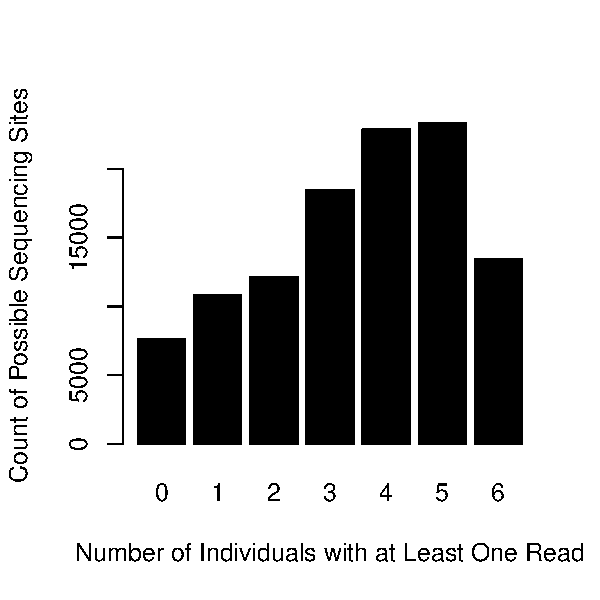
\includegraphics{figs/seq_site_coverage_by_ind}

\begin{itemize}
	\item SNP info from merged analysis
	\item SNP Venn diagram?
	\item Count orthologous SNPs shared between individuals
	\item VCFtools vcf-compare for this job
\end{itemize}

\section{Discussion}
\begin{itemize}
	\item RADseq is viable tool for researcher interested in primate phylogenetics, pop. gen.
	\item Enzyme choice allows control over coverage, number of individuals, number of loci.
	\item Potential problems with RADseq method
	\item Promise for primatology
\end{itemize}

\section{Acknowledgements}
Acknowledgements


\end{document}
